\documentclass{article}
\usepackage{graphicx} % Required for inserting images
\usepackage[top=0.9in, bottom=1in, left=1.5in, right=1.5in]{geometry}
\usepackage[utf8]{inputenc}
\usepackage[icelandic]{babel}
\usepackage[T1]{fontenc}
\usepackage[sc]{mathpazo}
\usepackage[parfill]{parskip}
\renewcommand{\baselinestretch}{1.2}
\usepackage{booktabs,tabularx}
\usepackage{multirow}
\usepackage{enumerate}
\usepackage{adjustbox}
\usepackage{multicol}
\usepackage{xcolor}
\usepackage{algpseudocode}
\usepackage{tikz}
\usepackage{nicefrac}
\usepackage{changepage}
\usetikzlibrary{arrows, positioning, calc, graphs}
\usepackage{amsmath, amsfonts, amssymb, amsthm}
\usepackage{graphicx}
\usepackage{tikz}
\usepackage{minted}
\usemintedstyle{manni}
\title{Forritunarmál Einstaklingsverkefni 11}
\author{Ragnar Björn Ingvarsson, rbi3}
\tikzset{->, >=stealth', shorten >=1pt, node distance=2cm,thick, main node/.style={circle,draw,minimum size=3em}}

\begin{document}
\renewcommand\thepage{}

	\maketitle

	\newpage
	\setcounter{page}{1}
	\renewcommand\thepage{\arabic{page}}

	\section{}
	\begin{minted}{haskell}
-- Notkun: listAll i n f
-- Fyrir:  i og n eru gildi af tagi af klasa Enum,
--         i <= n+1 og f er fall sem tekur inn eitt
--         viðfang af sama tagi.
-- Gildi:  Listinn [f(i),f(i+1),...,f(n)].
listAll i n f = map f [i..n]
	\end{minted}
	\begin{center}
		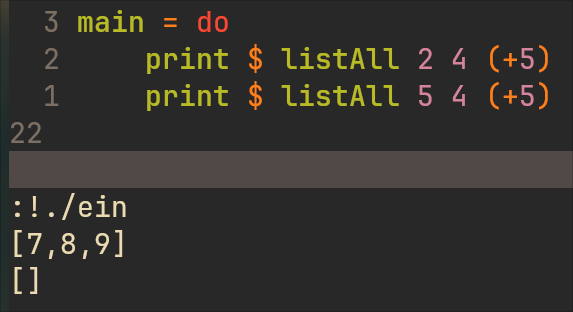
\includegraphics[scale=0.35]{listall.png}
	\end{center}

	\section{}
	\begin{minted}{haskell}
-- Notkun: powerList i j
-- Fyrir:  i og j eru heiltölur.
-- Gildi:  Listi allra mögulegra lista sem eru
--         undirlistar listans [i,i+1,...,j].
powerList i j
    | i > j     = [[]]
    | otherwise = powerList (i+1) j ++ (map (i:) $ powerList (i+1) j)
	\end{minted}
	\begin{center}
		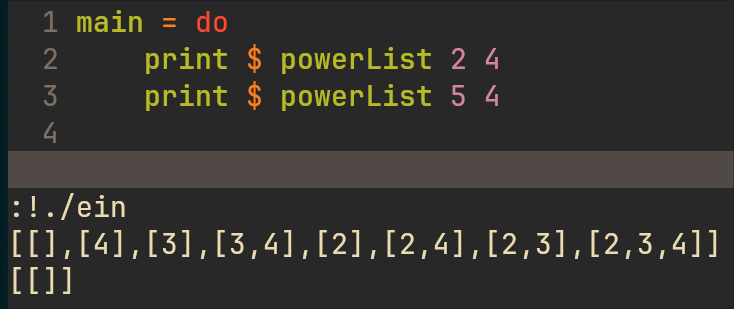
\includegraphics[scale=0.35]{powerlist.png}
	\end{center}
\end{document}
